\documentclass[oneside, final, 12pt]{extarticle}
\usepackage[T2A,T1]{fontenc}
\usepackage[utf8x]{inputenc}
\usepackage[english,russian]{babel}
\usepackage[usenames,dvipsnames]{xcolor}
\usepackage{listings}
\usepackage{xcolor}
\usepackage{lmodern}
\usepackage{textcomp}
\usepackage{lastpage}
\usepackage{vmargin}
\usepackage{titlesec}
\usepackage{mathptmx}
\usepackage{amsmath}
\usepackage{amssymb}
\usepackage{amsthm}
\usepackage{graphicx}
\usepackage{subfig}
\usepackage{pgf}
\usepackage{float}
\usepackage{titlesec}
\usepackage{cancel}
\usepackage{makecell}
\usepackage{float}
\usepackage{hyperref}

\allowdisplaybreaks

\floatstyle{plaintop}
\restylefloat{table}
\restylefloat{figure}

\titlelabel{\thetitle.\quad}

\graphicspath{ {./imgs/} }

\newcommand{\classname}[1]{\texttt{#1}}

\titlespacing*{\section}
{0pt}{5.5ex plus 1ex minus .2ex}{4.3ex plus .2ex}
\titlespacing*{\subsection}
{0pt}{5.5ex plus 1ex minus .2ex}{4.3ex plus .2ex}
\setpapersize{A4}
\setmarginsrb{2cm}{1.5cm}{1.5cm}{1.5cm}{0pt}{0mm}{0pt}{13mm}
\sloppy
\linespread{1.3}

\definecolor{mGreen}{rgb}{0,0.6,0}
\definecolor{mPurple}{rgb}{0.58,0,0.82}
\definecolor{maroon}{rgb}{0.5,0,0}
\definecolor{darkgreen}{rgb}{0,0.5,0}
\definecolor{darkbrown}{RGB}{139,69,19}
\definecolor{darkblue}{RGB}{25,25,112}

\lstdefinestyle{CStyle}{,   
    commentstyle=\color{mGreen},
    keywordstyle=\color{magenta},
    stringstyle=\color{mPurple},
    basicstyle=\footnotesize,
    breakatwhitespace=false,         
    breaklines=true,                 
    captionpos=b,                    
    keepspaces=true,                 
    showspaces=false,                
    showstringspaces=false,
    showtabs=false,                  
    tabsize=2,
    language=C
}

\lstdefinelanguage{INI}
{
  basicstyle=\ttfamily\footnotesize,
  morecomment=[l]{;},
  morecomment=[s][\color{darkblue}\bfseries]{[}{]},
  moredelim=[s][\color{darkbrown}]{=}{\ },
  commentstyle=\color{darkgreen},
  keywordstyle={\color{maroon}\bfseries},
  morekeywords={param,parameter,parameter2}
}

\begin{document}

\normalsize

\begin{titlepage}
    \begin{center}
        \textsc{Московский Государственный Университет имени М.В. Ломоносова\\[5mm]
            Факультет вычислительной математики и кибернетики}
        \centerline{\hfill\hrulefill\hrulefill\hfill}
    \end{center}

    \vfill
    \vfill
    \vfill
    \vfill
    \begin{center}
        \Large
        \textbf{Отчёт по практическому заданию 3 \\
            в рамках курса
            «Суперкомпьютерное моделирование и технологии»}
    \end{center}

    \vfill
    \vfill
    \vfill
    \hfill
    \begin{flushright}
        Вариант 8
    \end{flushright}

    \begin{flushright}
        Выполнил: \\
        Шорошов Григорий Максимович, \\
        622 группа \\[5mm]
    \end{flushright}

    \vfill
    \vfill
    \vfill
    \begin{center}
        Москва, \the\year
    \end{center}
\end{titlepage}

\parindent=1cm

\newpage
\section{Математическая постановка задачи}

В трехмерной замкнутой области
$$
\Omega = [0 \leq x \leq L_x] \times [0 \leq y \leq L_y] \times [0 \leq z \leq L_z] 
$$
для $ (0 < t \leq T] $ требуется найти решение $ u(x, y, z, t) $ уравнения в частных производных
\begin{align}
\frac{\partial^2 u}{\partial t^2} = \bigtriangleup u \label{eqn:main}
\end{align}

с начальными условиями
\begin{align}
& u|_{t = 0} = \phi(x, y, z) \label{eqn:condition1} \\
& \frac{\partial u}{\partial t}|_{t = 0} = 0 \label{eqn:condition2}
\end{align}
при условии, что на границах области заданы однородные граничные условия первого рода
\begin{align}
& u(0, y, z, t) = 0, \qquad \qquad u(L_x, y, z, t) = 0 \\
& u(x, 0, z, t) = 0, \qquad \qquad u(x, L_y, z, t) = 0 \\
& u(x, y, 0, t) = 0, \qquad \qquad u(x, y, L_z, t) = 0
\end{align}
либо периодические условия
\begin{align}
& u(0, y, z, t) = u(L_x, y, z, t) \qquad \qquad u_x(0, y, z, t) = u_x(L_x, y, z, t) \label{eqn:period1} \\
& u(x, 0, z, t) = u(x, L_y, z, t) \qquad \qquad u_y(x, 0, z, t) = u_y(x, L_y, z, t) \label{eqn:period2} \\
& u(x, y, 0, t) = u(x, y, L_z, t) \qquad \qquad u_z(x, y, 0, t) = u_z(x, y, L_z, t) \label{eqn:period3}
\end{align}
Был реализован вариант 8 для функции
$$
u(x, y, z, t) = \sin(\frac{2 \pi}{L_x} x) \cdot \sin(\frac{4 \pi}{L_y} y) \cdot \sin(\frac{6 \pi}{L_z} z)
\cdot \cos(a_t \cdot t), \: a_t = \pi \sqrt{\frac{4}{L_x^2} + \frac{16}{L_y^2} + \frac{36}{L_z^2}} 
$$
и периодических граничных условий.

\section{Численный метод решения задачи}

Для численного решения задачи введем на $ \Omega $ сетку $ \omega_{h \tau} = \overline{\omega_h} \times \omega_{\tau} $, где
\begin{align*}
& T = T_0, \\
& L_x = L_{x_0}, \: L_y = L_{y_0}, \: L_z = L_{z_0}, \\
& \overline{\omega_h} = \{ ( x_i = i h_x, y_J = j h_y, z_k = k h_z ), \: i, j, k = 0, 1, ..., N, \: h_x N = L_x, \: h_y N = L_y, \: h_z N = L_z \}, \\
& \omega_{\tau} = \{ t_n = n \tau, \: n = 0, 1, ..., K, \: \tau K = T \}.
\end{align*}

Через $ \omega_h $ обозначим множество внутренних, а через $ \gamma_h $ --- множество граничных узлов сетки $ \overline{\omega_h} $.

Для аппроксимации исходного уравнения (\ref{eqn:main}) воспользуемся следующей системой уравнений:
\begin{align}
\frac{u_{ijk}^{n + 1} - 2u_{ijk}^{n} + u_{ijk}^{n - 1} }{\tau ^ 2} = \bigtriangleup_h u^n, \: (x_i, y_j, z_k) \in \omega_h, \: n = 1, 2, ..., K - 1, \label{eqn:approx}
\end{align}
где $ \bigtriangleup_h $ --- разностный аналог оператора Лапласа:
$$
\bigtriangleup_h u^n = \frac{u^n_{i - 1, j, k} - 2u^n_{i, j, k} + u^n_{i + 1, j, k}}{h^2} + 
\frac{u^n_{i, j - 1, k} - 2u^n_{i, j, k} + u^n_{i, j + 1, k}}{h^2} + 
\frac{u^n_{i, j, k - 1} - 2u^n_{i, j, k} + u^n_{i, j, k + 1}}{h^2}.
$$

Значения $u^{n + 1}_{i,j,k}$ можно явным образом выражаются через значения на n-м и (n-1)-м шаге. 

Зададим значения $ u_{i, j, k}^{0}, u_{i, j, k}^{1}, \: (x_i, y_j, z_k) \in \omega_h $, исходя из условий (\ref{eqn:condition1}) и (\ref{eqn:condition2}):
\begin{align}
& u^0_{i,j,k} = \phi(x_i, y_j, z_k), \: (x_i, y_j, z_k) \in \omega_h \\
& u^1_{i,j,k} = u^0_{i,j,k} + \frac{\tau ^ 2}{2}  \bigtriangleup_h \phi(x_i, y_j, z_k) \label{eqn:u1}
\end{align}

Разностная аппроксимация для периодических граничных условий (\ref{eqn:period1})--(\ref{eqn:period3}) выглядит следующим образом:
\begin{align*}
& u^{n + 1}_{0,j,k} = u^{n + 1}_{N,j,k} = \frac{u^{n + 1}_{1,j,k} + u^{n + 1}_{N - 1,j,k}}{2} \\
& u^{n + 1}_{i,0,k} = u^{n + 1}_{i,N,k} = \frac{u^{n + 1}_{i,1,k} + u^{n + 1}_{i,N - 1,k}}{2} \\
& u^{n + 1}_{i,j,0} = u^{n + 1}_{i,j,N} = \frac{u^{n + 1}_{i,j,1} + u^{n + 1}_{i,j,N - 1}}{2}
\end{align*}

\section{Описание программной реализации}

Код решения можно найти по \href{https://github.com/shorohml/SuperComp/tree/master/task3}{ссылке}.

Конфигурация запуска хранится в формате INI, для чтения конфигурации использовалась библиотека \href{https://github.com/jtilly/inih}{inih}.
Пример файла конфигурации:
\begin{lstlisting}[language={INI}]
[Solver]
    L_x=1.0
    L_y=1.0
    L_z=1.0
    N_x=128
    N_y=128
    N_z=128
    periodic_x=true
    periodic_y=true
    periodic_z=true
    K=20
    T=0.025
    print_layer_err=true
    save_layers=false
    save_step=5
    layers_path=./layers/    
\end{lstlisting}

Данные из файла считывает объект класса \classname{Config}, который создается в конструкторе класса \classname{Solver}.
Далее в конструкторе \classname{Solver}:
\begin{itemize}
    \item выполняем команду
    \begin{lstlisting}[style=CStyle]
        MPI_Init(&argc, &argv);
    \end{lstlisting}
    \item запрашиваем количество запущенных MPI процессов и свой номер:
    \begin{lstlisting}[style=CStyle]
        MPI_Comm_rank(MPI_COMM_WORLD, &rank);
        MPI_Comm_size(MPI_COMM_WORLD, &size);
    \end{lstlisting}
    \item определяем сбалансированное распределение процессов по решетке, создаем виртуальную топологию и определяем координаты процессора в решетке:
    \begin{lstlisting}[style=CStyle]
        MPI_Dims_create(size, 3, dims);
        MPI_Cart_create(MPI_COMM_WORLD, 3, dims, 
                        config.periodic, true, &comm);
        MPI_Cart_coords(comm, rank, 3, coords);
    \end{lstlisting}    
    \item вычисляем размеры и координаты блока решетки $ \overline{\omega_h} $, за который отвечает процессор:
    \begin{lstlisting}[style=CStyle]
        compute_block_coords();
    \end{lstlisting}
    \item выделяем память (вызывая метод resize) под блоки на шагах n + 1, n, n - 1 алгоритма, блоки для хранения погрешности и аналитического решения, а также под значения,
    пересылаемые из соседних процессов:
    \begin{lstlisting}[style=CStyle]
        Block3D<double> blocks[3];
        Block3D<double> errs;
        Block3D<double> analytical;
        Block3DBound<double> bound;    
    \end{lstlisting}
    \item создаем типы для передачи граней блока соседним процессам.
\end{itemize}

Для хранения блоков используются класс \classname{Block3D}, который содержит размер блока, его координаты
 и узлы решетки, которые хранятся в объекте класса \classname{Grid3D}. Элементы решетки хранятся 
 в объекте класса \classname{std::vector<double>} размера \classname{P\_x * P\_y * P\_z}.
 Доступ к элементам решетки происходит через вызов оператора \classname{operator()(int i, int j, int k)}.

Каждому процессу соответствует один блок. Расчет внутренних элементов блока не зависит от соседних блоков и
векторизуется через \classname{pragma omp parallel for}.
Однако для расчета граничных элементов блока необходимо:
\begin{itemize}
\item получить граничные элементы соседних блоков $ u^n $;
\item если граница блока совпадает с границей области $ \Omega $, получить
$ u^{n + 1}_{1,j,k}, u^{n + 1}_{N - 1,j,k}, u^{n + 1, }_{i,1,k}, u^{n + 1}_{1,N - 1,k}, u^{n + 1}_{i,j,1}, u^{n + 1}_{i,j,N - 1} $.
\end{itemize}

Пересылка граничных элементов блоков реализована в методах \classname{send\_inner\_values} (для внутренних узлов сетки) и \classname{send\_boundary\_values}
(для граничных узлов сетки). Алгоритм пересылки следующий:
\begin{itemize}
    \item по каждой оси выполняется асинхронная отправка граней своего блока соседним процессам;
    \item для каждой оси выполняется блокирующее получение граней блоков соседних процессов;
    \item процесс дожидается завершения отправок.
\end{itemize}

Вычисление разностной схемы происходит в методе \classname{run} класса \classname{Solver}. Алгоритм работы следующий:
\begin{itemize}
    \item рассчитываются аналитические значения на 0 слое;
    \item рассчитывается 1 слой по формуле (\ref{eqn:u1});
    \item для всех $ t_n, \: 2 \leq n \leq K $:
    \begin{itemize}
    \item рассчитывается 2 слой по формуле (\ref{eqn:approx});
    \item вычисляется максимальная погрешность на слое;
    \item если в конфигурации задано сохранение слоя, то слой сохраняется на диск.
    \end{itemize}
\end{itemize}

В деструкторе класса \classname{Solver}:
\begin{itemize}
    \item вычисляем наибольшее время выполнение среди всех процессов и выводим его;
    \item вызываем \classname{MPI\_Finalize}.
\end{itemize}

\section{Графики аналитического, посчитанного решений и погрешности}

\begin{figure}[H]
    \centering
    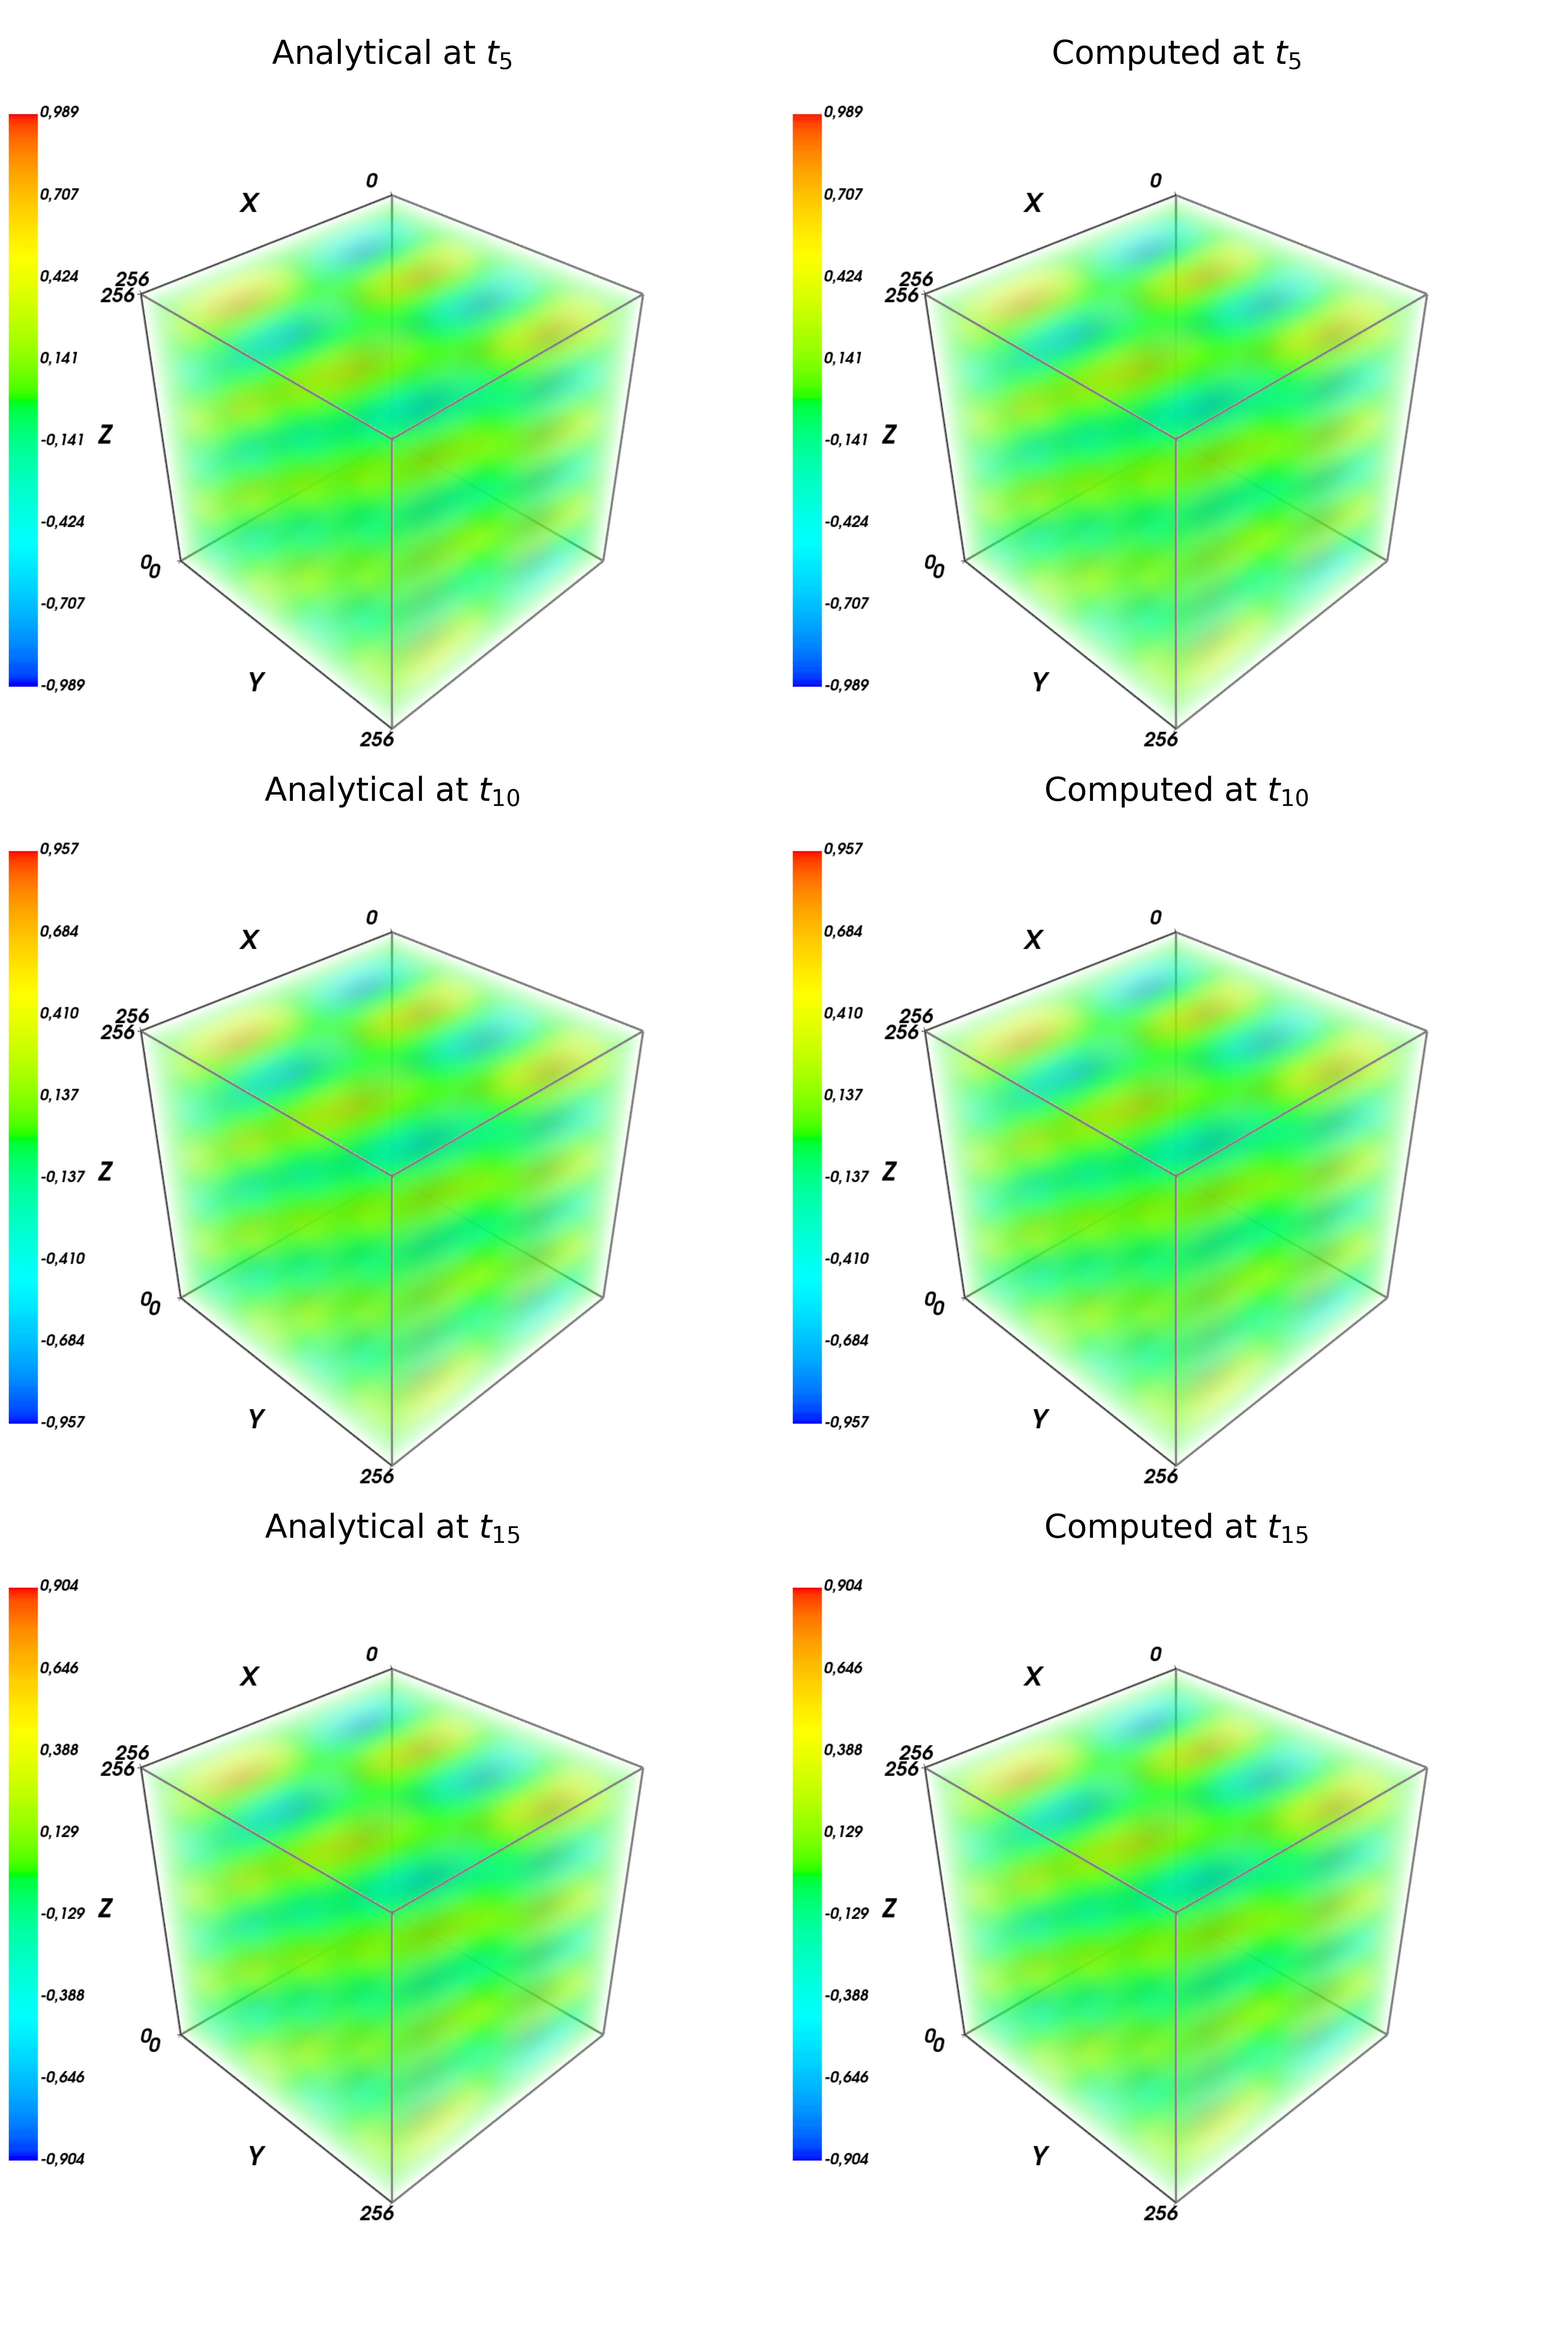
\includegraphics[width=0.8\textwidth]{cmp.png}
    \caption{Аналитическое и посчитанное решения для $ N = 256, \: T = 0.025, \: L_x = L_y = L_z = 1.0 $}
\end{figure}

\begin{figure}[H]
    \centering
    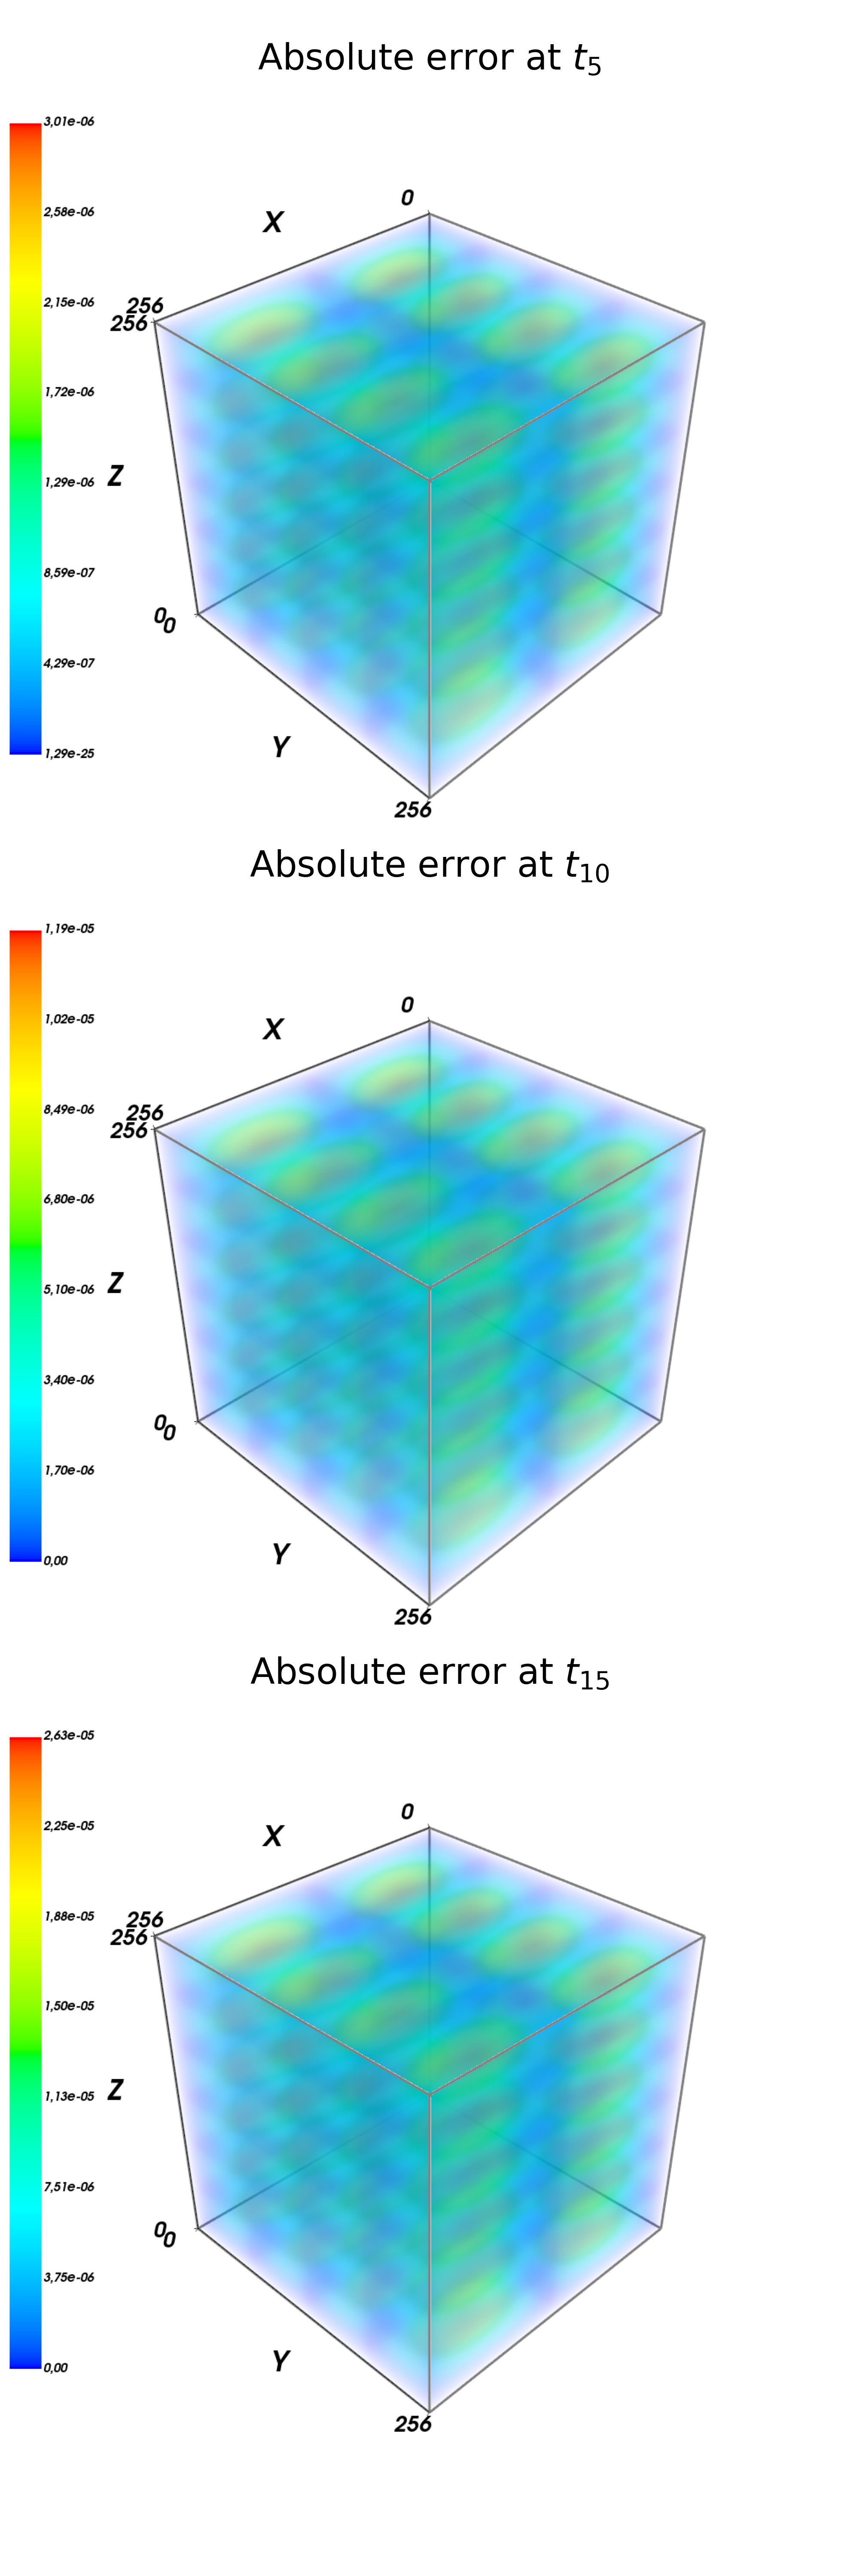
\includegraphics[width=0.5\textwidth]{errs.png}
    \caption{Погрешность решения для $ N = 256, \: T = 0.025, \: L_x = L_y = L_z = 1.0 $}
\end{figure}

\section{Результаты расчетов}

Запуски программы проведены на системах Blue Gene/P и Polus для:
\begin{itemize}
    \item $ L_x = L_y = L_z = 1.0, \: K = 20, \: T = 0.025 $
    \item $ L_x = L_y = L_z = \pi, \: K = 20, \: T = 0.025 $
\end{itemize}

Запуски на Blue Gene/P проводились в режиме SMP.
Гибридная версия программы MPI/OpenMP запускалась на BlueGene/P с OMP \_NUM\_THREADS=4.

\begin{table}[H]
    \centering
    \begin{tabular}{|l|l|l|l|l|}
        \hline
        \makecell{Число точек \\сетки $ N^3 $} & \makecell{Число \\процессоров $ N_p $} & \makecell{Время \\решения $ T_s $} & Ускорение $ S $ & Погрешность $ \delta $ \\
        \hline
        $ 128^3 $                 & 10               & 0.500 & 1.000  & 0.000217197 \\
        \cline{2-4}
                              & 20               & 0.481 & 1.041  & \\
        \cline{2-4}
                              & 40              & 0.305 & 1.640 & \\
        \hline
        $ 256^3 $                 & 10               & 3.214 & 1.000  & 4.55295e-05 \\
        \cline{2-4}
                              & 20               & 2.211 & 1.454  & \\
        \cline{2-4}
                              & 40              & 1.520 & 1.920  & \\
        \hline
        $ 512^3 $                 & 10               & 25.770 & 1.000  & 2.58835e-06 \\
        \cline{2-4}
                              & 20               & 16.955 & 1.520 & \\
        \cline{2-4}
                              & 40              & 10.276 & 2.741 & \\
        \hline
    \end{tabular}
    \caption{Таблица с результатами расчётов для системы Polus, $ L_x = L_y = L_z = 1.0, \: K = 20, \: T = 0.025 $}
\end{table}

\begin{table}[H]
    \centering
    \begin{tabular}{|l|l|l|l|l|}
        \hline
        \makecell{Число точек \\сетки $ N^3 $} & \makecell{Число \\процессоров $ N_p $} & \makecell{Время \\решения $ T_s $} & Ускорение $ S $ & Погрешность $ \delta $ \\
        \hline
        $ 128^3 $                 & 10               & 0.503 & 1.000  & 2.43122e-05 \\
        \cline{2-4}
                              & 20               & 0.458 & 1.046  & \\
        \cline{2-4}
                              & 40              & 0.380 & 1.649 & \\
        \hline
        $ 256^3 $                 & 10               & 3.216 & 1.000  & 5.98586e-06 \\
        \cline{2-4}
                              & 20               & 2.540 & 1.454  & \\
        \cline{2-4}
                              & 40              & 1.674 & 2.115 & \\
        \hline
        $ 512^3 $                 & 10               & 25.325 & 1.000  & 1.4015e-06 \\
        \cline{2-4}
                              & 20               & 16.852 & 1.520 & \\
        \cline{2-4}
                              & 40              & 9.401 & 2.508 & \\
        \hline
    \end{tabular}
    \caption{Таблица с результатами расчётов для системы Polus, $ L_x = L_y = L_z = \pi, \: K = 20, \: T = 0.025 $}
\end{table}

\begin{table}[H]
    \centering
    \begin{tabular}{|l|l|l|l|l|l|l|l|}
        \hline
        \makecell{$ N^3 $} & \makecell{$ N_p $} 
        & \makecell{Время \\решения \\$ T_{MPI} $} & \makecell{Ускорение \\$ S_{MPI} $} 
        & \makecell{Время \\решения \\$ T_{MPI\_OpenMP} $} & \makecell{Ускорение \\$ S_{MPI\_OpenMP} $}
        & \makecell{$ \frac{ T_{MPI} }{ T_{MPI\_OpenMP} } $}
        & Погрешность $ \delta $ \\
        \hline
        128 & 64 & 1.243 & 1.000 & 0.403 & 3.084 & 3.084 & 0.000217197\\
        \cline{2-7}
         & 128 & 0.663 & 1.874 & 0.240 & 5.174 & 2.761 & \\
        \cline{2-7}
         & 512 & 0.189 & 6.564 & 0.078 & 16.014 & 2.440 & \\
        \hline
        256 & 64 & 9.248 & 1.000 & 2.812 & 3.288 & 3.288 & 4.55295e-05\\
        \cline{2-7}
         & 128 & 4.777 & 1.936 & 1.514 & 6.110 & 3.156 & \\
        \cline{2-7}
         & 512 & 1.252 & 7.389 & 0.407 & 22.735 & 3.077 & \\
        \hline
        512 & 64 & 71.109 & 1.000 & 21.007 & 3.385 & 3.385 & 2.58822e-06\\
        \cline{2-7}
         & 128 & 36.101 & 1.970 & 10.842 & 6.559 & 3.330 & \\
        \cline{2-7}
         & 512 & 9.225 & 7.709 & 2.789 & 25.495 & 3.307 & \\
        \hline               
    \end{tabular}
    \caption{Таблица с результатами расчётов для системы Blue Gene/P, $ L_x = L_y = L_z = 1.0, \: K = 20, \: T = 0.025 $}
\end{table}

\begin{table}[H]
    \centering
    \begin{tabular}{|l|l|l|l|l|l|l|l|}
        \hline
        \makecell{$ N^3 $} & \makecell{$ N_p $} 
        & \makecell{Время \\решения \\$ T_{MPI} $} & \makecell{Ускорение \\$ S_{MPI} $} 
        & \makecell{Время \\решения \\$ T_{MPI\_OpenMP} $} & \makecell{Ускорение \\$ S_{MPI\_OpenMP} $}
        & \makecell{$ \frac{ T_{MPI} }{ T_{MPI\_OpenMP} } $}
        & Погрешность $ \delta $ \\
        \hline
        128 & 64 & 1.208 & 1.000 & 0.394 & 3.070 & 3.070 & 2.43122e-05\\
        \cline{2-7}
         & 128 & 0.644 & 1.877 & 0.235 & 5.136 & 2.735 & \\
        \cline{2-7}
         & 512 & 0.185 & 6.522 & 0.077 & 15.742 & 2.414 & \\
        \hline
        256 & 64 & 8.938 & 1.000 & 2.739 & 3.263 & 3.263 & 5.98586e-06\\
        \cline{2-7}
         & 128 & 4.619 & 1.935 & 1.477 & 6.050 & 3.126 & \\
        \cline{2-7}
         & 512 & 1.217 & 7.346 & 0.396 & 22.556 & 3.070 & \\
        \hline
        512 & 64 & 68.650 & 1.000 & 20.394 & 3.366 & 3.366 & 1.4015e-06\\
        \cline{2-7}
         & 128 & 34.872 & 1.969 & 10.544 & 6.511 & 3.307 & \\
        \cline{2-7}
         & 512 & 8.927 & 7.690 & 2.711 & 25.319 & 3.292 & \\
        \hline        
    \end{tabular}
    \caption{Таблица с результатами расчётов для системы Blue Gene/P, $ L_x = L_y = L_z = \pi, \: K = 20, \: T = 0.025 $}
\end{table}

\end{document}